\chapter{Risultati sperimentali}
\textit{In questo capitolo verrà analizzata l'applicazione ponendo l'attenzione sul software usato per eseguire il docking e successivamente saranno anilzzate le prestazioni dell'applicazione nel complessivo prendendo in esame i tempi di esecuzione dei moduli che compongono l'applicativo.}

\vskip 1cm

\section{I casi di analisi}
I dati prodotti dall'applicazione soddisfano gli obbiettivi preposti, per effettuare un'analisi migliore delle prestazioni e delle capacità di \textbf{AUDO4RIAS}, è stato stressato il modulo principale del software ovvero il modulo del docking, confrontando lo strumento software utilizzato dall'applicativo trattato, \textbf{AutoDock Vina}, con un altro strumento software per eseguire il docking, \textbf{GNINA}.\newline
I dati e parte dei risultati sperimentali sono stati ottenuti dallo studio effettuato dal mio collega Orsini, parte importante della sua tesi riguardava proprio il confronto dei due software. A tal riguardo è possibile ottenere maggiori informazioni tramite il seguente link: \url{https://github.com/gomax22/bachelor-thesis}.\newline
Le prestazioni sono state riportate a vari livelli di profondità, partendo da una prima considerazione visuale della posa del ligando predetta, arrivando a motivare e valutare i valori osservati per le caratteristiche riportate. Le proteine selezionate per l’analisi dei risultati del docking effettuato tra i due software sopracitati sono le proteine: \textit{1FCU, 2H8V, 3FE9, 4E81, 5XZ3\_A e 6LQK\_B}, per queste proteine sono state scelte le pose con i ligandi: \textit{Acrinathrin, Dimethomorph, Glyphosate e Oxyfluorfen}.\newline
Le proteine precedentemente citate sono state scelte in quanto si differenziano per dimensione e conformazione, offrendo maggiore varietà dei casi di esame.\newline
Per fornire un'analisi complessiva di \textbf{AUDO4RIAS}, infine, sono stati analizzati i tempi di esecuzione dei moduli che compongono il software.

\section{GNINA}
\textbf{GNINA} è un software per l'esecuzione del docking, che utilizza un insieme di reti neurali convoluzionali (CNN) come funzione di scoring. Le prestazioni del docking, sono valutate confrontando lo scoring ottenuto da GNINA con quello di AutoDock Vina quando si utilizzano tasche di legame esplicitamente definite o proteine intere. GNINA, utilizzando una funzione di punteggio CNN per ricalibrare le pose in uscita, supera il punteggio di AutoDock Vina nei compiti di redocking e cross-docking quando la tasca di legame è definita (aumenta dal 58\% al 73\% e dal 27\% al 37\%, rispettivamente) e quando è l'intera proteina a definire la tasca di legame (aumenta dal 31\% al 38\% e dal 12\% al 16\%, rispettivamente). Di seguito il repository di GNINA con licenza open source per l'uso come strumento di docking molecolare: \url{https://github.com/gnina/gnina}.\cite{mcnutt2021gnina}

\section{Visualizzazione della predizione della posa}
Il primo termine di confronto tra AutoDock Vina e GNINA sono le pose predette, sono state fatte calcolare ad entrambi le pose per ogni proteina sopracitata, queste sono poi state analizzate utilizzando la suite \textbf{AutoDockTools} trattata nella sezione \ref{AutoDockTools}.\newline
Solo le pose migliori predette da entrambi i software sono state analizzate, per cui le differenze riscontrate possono essere imputate alla randomicità del calcolo delle pose, ai diversi criteri adottati da ciascun software e da eventuali filtri applicati. 

\begin{figure}[H]
    \centering
    \begin{subfigure}[b]{0.475\textwidth}
        \centering
        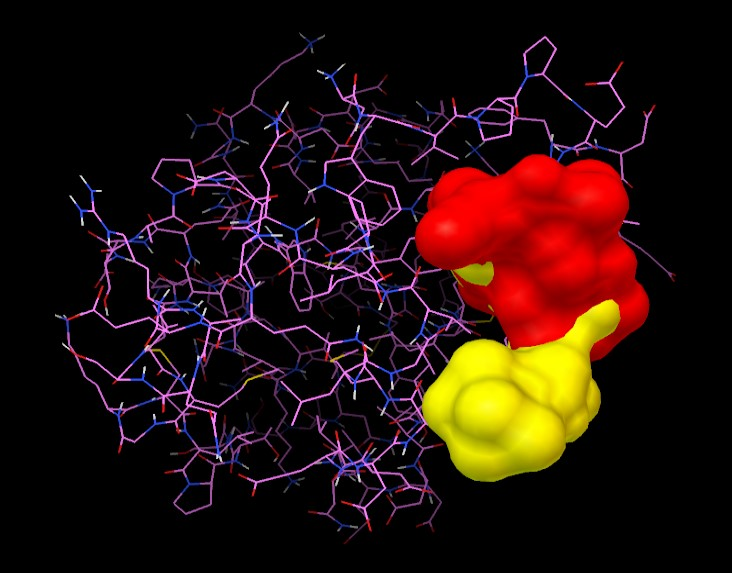
\includegraphics[width=\textwidth, height=6cm]{immagini/capitolo4/2h8v_acrinathrin.jpg}
        \caption[]%
        {{\small Acrinathrin}}    
        \label{fig:2h8v_acrinathrin}
    \end{subfigure}
    \hfill
    \begin{subfigure}[b]{0.475\textwidth}  
        \centering 
        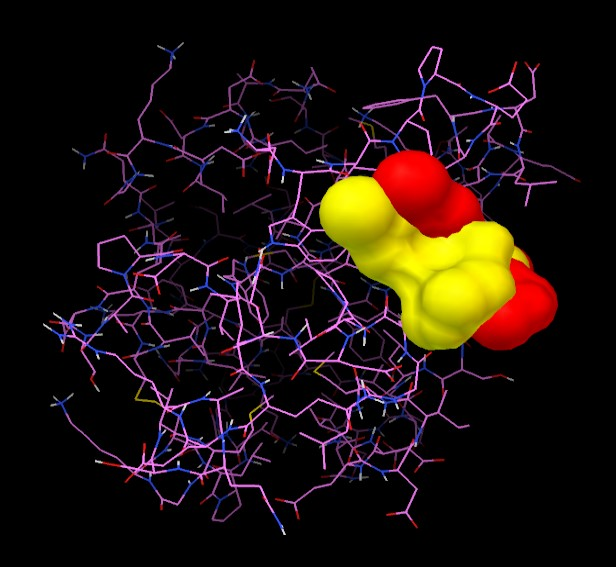
\includegraphics[width=\textwidth, height=6cm]{immagini/capitolo4/2h8v_dimethomorph.jpg}
        \caption[]%
        {{\small Dimethomorph}}    
        \label{fig:2h8v_dimethomorph}
    \end{subfigure}
    \vskip\baselineskip
    \begin{subfigure}[b]{0.475\textwidth}   
        \centering 
        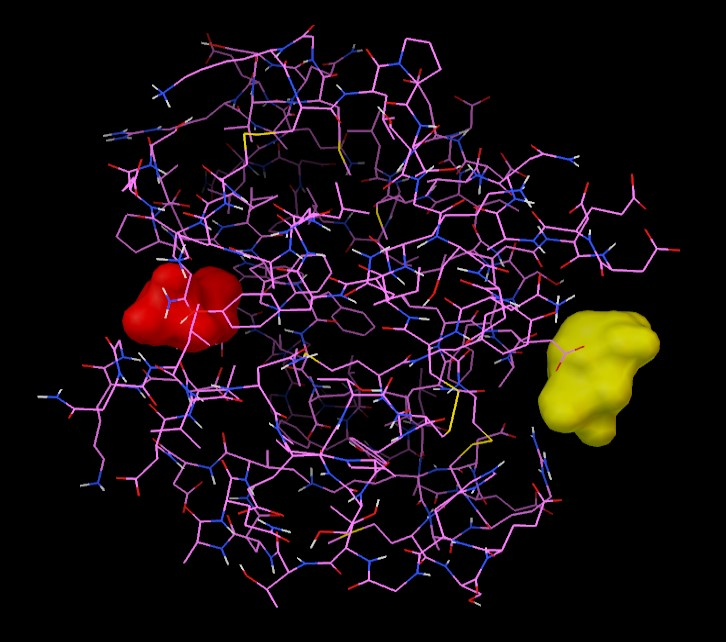
\includegraphics[width=\textwidth, height=6cm]{immagini/capitolo4/2h8v_glyphosate.jpg}
        \caption[]%
        {{\small Glyphosate}}    
        \label{fig:2h8v_glyphosate}
    \end{subfigure}
    \hfill
    \begin{subfigure}[b]{0.475\textwidth}   
        \centering 
        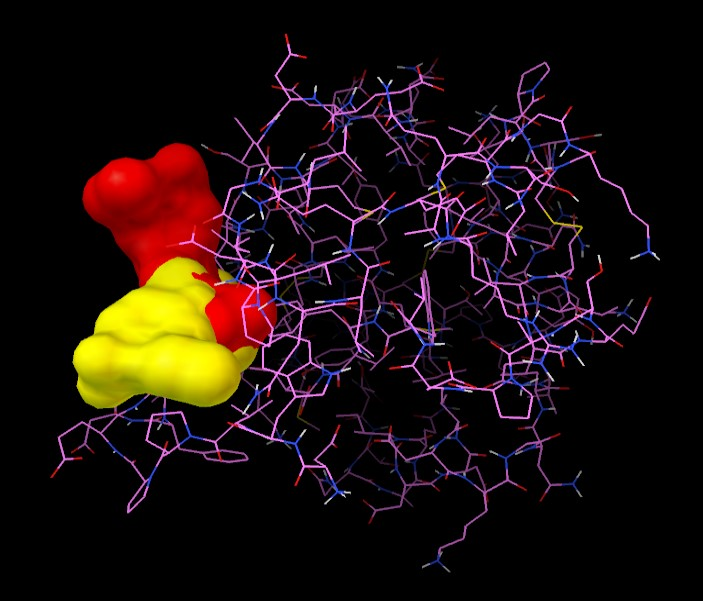
\includegraphics[width=\textwidth, height=6cm]{immagini/capitolo4/2h8v_oxyfluorfen.jpg}
        \caption[]%
        {{\small Oxyfluorfen}}    
        \label{fig:2h8v_oxyfluorfen}
    \end{subfigure}
    \caption[Conformazioni proteina-ligando per la proteina 2H8V]
    {\small Visualizzazione delle migliori pose generate da GNINA (in giallo) ed AutoDock Vina (in rosso) relativamente alla proteina 2H8V ed alcuni dei ligandi del dataset iniziale (Acrinathrin, Dimethomorph, Glyphosate, Oxyfluorfen).} 
    \label{fig:2h8v}
\end{figure}

Nella foto \ref{fig:2h8v} sono mostrate le migliori pose calcolate da AutoDock Vina e da GNINA per la proteina \textit{2h8v}, questa è caratterizzata da piccole dimensioni, osservando il sito di legame relativo alle migliori pose predette si può concludere come il sito di legame individuato dai due software sia sostanzialmente lo stesso, a meno di orientazioni e torsioni del ligando coinvolto. Possiamo concludere che per recettori di piccole dimensioni le predizioni di AutoDock e di GNINA sono piuttosto simili, sebbene abbiano configurazioni differenti.

\begin{figure}[H]
    \centering
    \begin{subfigure}[b]{0.475\textwidth}
        \centering
        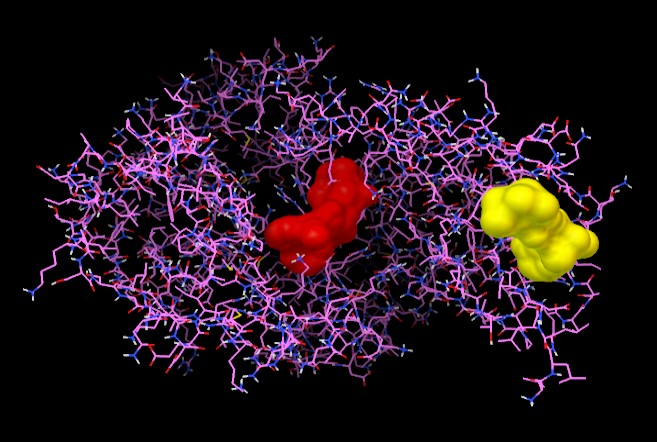
\includegraphics[width=\textwidth, height=6cm]{immagini/capitolo4/4e81_acrinathrin.jpg}
        \caption[]%
        {{\small Acrinathrin}}    
        \label{fig:4e81_acrinathrin}
    \end{subfigure}
    \hfill
    \begin{subfigure}[b]{0.475\textwidth}  
        \centering 
        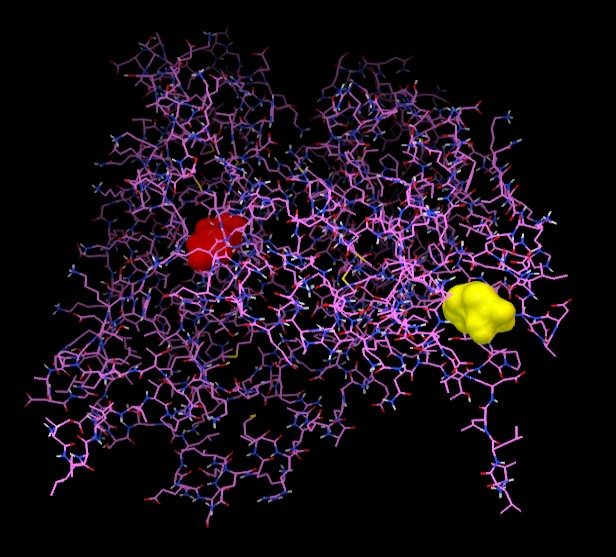
\includegraphics[width=\textwidth, height=6cm]{immagini/capitolo4/4e81_glyphosate.jpg}
        \caption[]%
        {{\small Dimethomorph}}    
        \label{fig:4e81_dimethomorph}
    \end{subfigure}
    \vskip\baselineskip
    \begin{subfigure}[b]{0.475\textwidth}   
        \centering 
        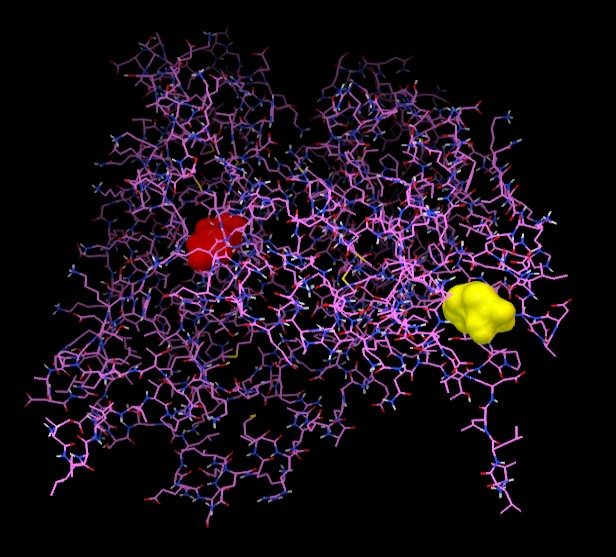
\includegraphics[width=\textwidth, height=6cm]{immagini/capitolo4/4e81_glyphosate.jpg}
        \caption[]%
        {{\small Glyphosate}}    
        \label{fig:4e81_glyphosate}
    \end{subfigure}
    \hfill
    \begin{subfigure}[b]{0.475\textwidth}   
        \centering 
        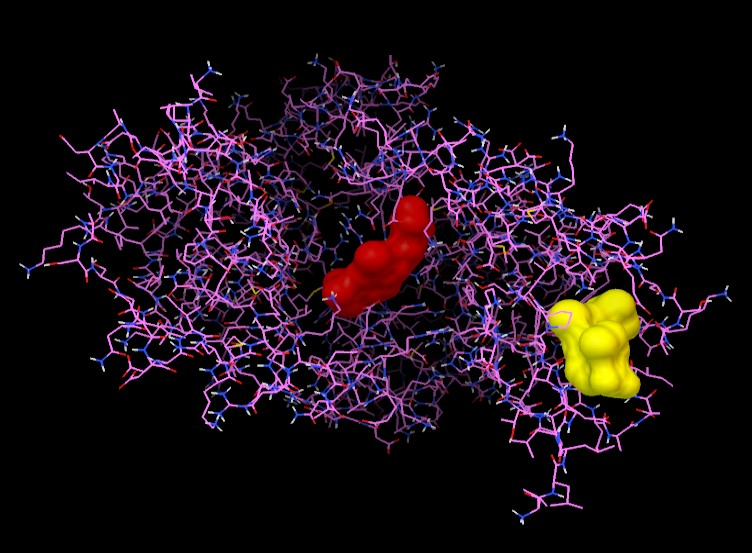
\includegraphics[width=\textwidth, height=6cm]{immagini/capitolo4/4e81_oxyfluorfen.jpg}
        \caption[]%
        {{\small Oxyfluorfen}}    
        \label{fig:4e81_oxyfluorfen}
    \end{subfigure}
    \caption[Conformazioni proteina-ligando per la proteina 4E81.]
    {\small Visualizzazione delle migliori pose generate da GNINA (in giallo) ed AutoDock Vina (in rosso) relativamente alla proteina 4E81 ed alcuni dei ligandi del dataset iniziale (Acrinathrin, Dimethomorph, Glyphosate, Oxyfluorfen).} 
    \label{fig:4e81}
\end{figure}

Se si analizza un caso differente, quale le pose calcolate per la proteina \textit{4E81}, mostrate nella figura \ref{fig:4e81}, si nota una notevole differenza nelle predizioni: nel caso di GNINA, il ligando risulta occupare una posizione quasi esterna alla proteina mentre è tendenzialmente interna nel caso di AutoDock Vina.

\begin{figure}[H]
    \centering
    \begin{subfigure}[b]{0.475\textwidth}
        \centering
        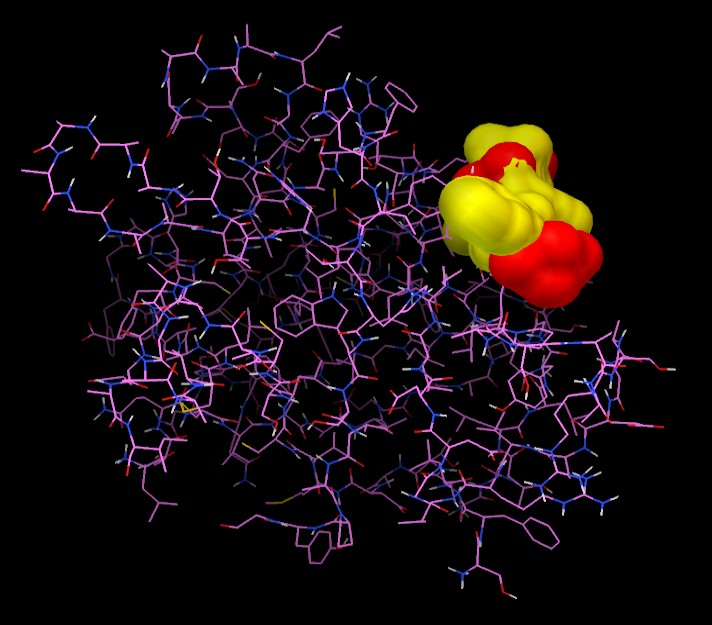
\includegraphics[width=\textwidth, height=6cm]{immagini/capitolo4/6lqk_b_acrinathrin.jpg}
        \caption[]%
        {{\small Acrinathrin}}    
        \label{fig:6lqk_b_acrinathrin}
    \end{subfigure}
    \hfill
    \begin{subfigure}[b]{0.475\textwidth}  
        \centering 
        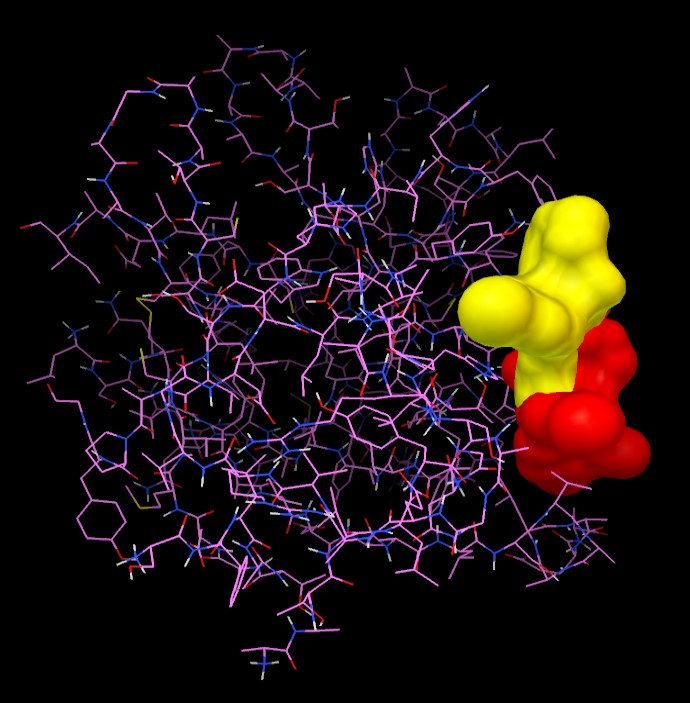
\includegraphics[width=\textwidth, height=6cm]{immagini/capitolo4/6lqk_b_dimethomorph.jpg}
        \caption[]%
        {{\small Dimethomorph}}    
        \label{fig:6lqk_b_dimethomorph}
    \end{subfigure}
    \vskip\baselineskip
    \begin{subfigure}[b]{0.475\textwidth}   
        \centering 
        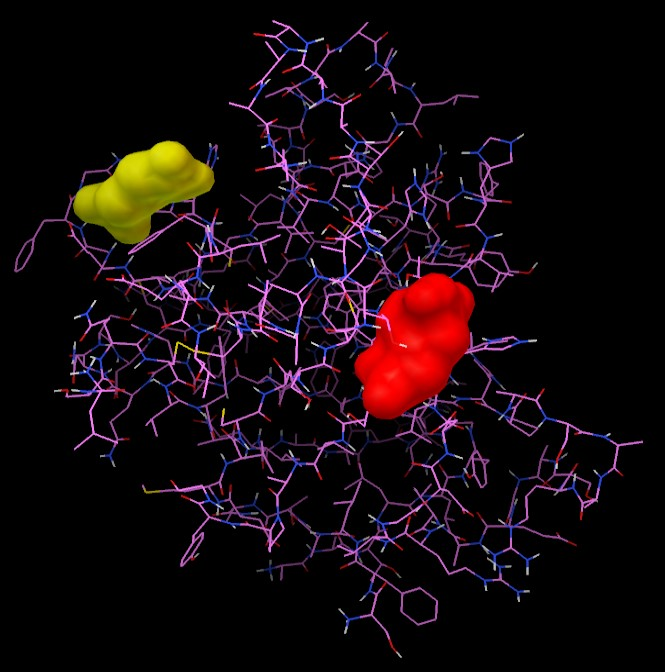
\includegraphics[width=\textwidth, height=6cm]{immagini/capitolo4/6lqk_b_glyphosate.jpg}
        \caption[]%
        {{\small Glyphosate}}    
        \label{fig:6lqk_b_glyphosate}
    \end{subfigure}
    \hfill
    \begin{subfigure}[b]{0.475\textwidth}   
        \centering 
        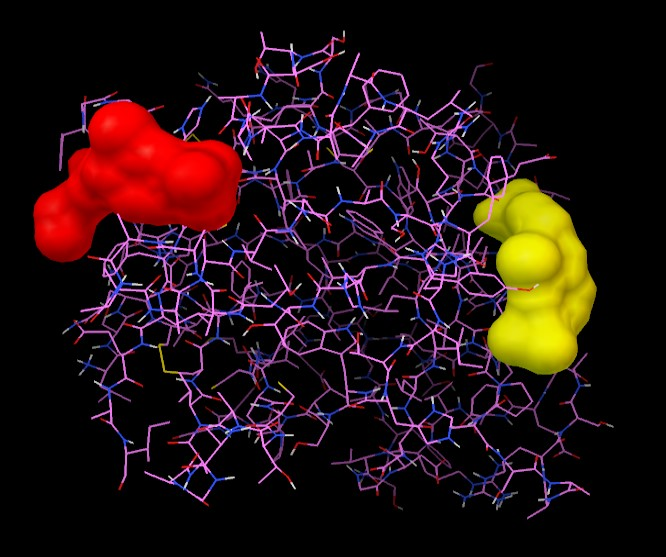
\includegraphics[width=\textwidth, height=6cm]{immagini/capitolo4/6lqk_b_oxyfluorfen.jpg}
        \caption[]%
        {{\small Oxyfluorfen}}    
        \label{fig:6lqk_b_oxyfluorfen}
        \end{subfigure}
    \caption[Conformazioni proteina-ligando per la proteina 6LQK\_B]
    {\small Visualizzazione delle migliori pose generate da GNINA (in giallo) ed AutoDock Vina (in rosso) relativamente alla proteina 6LQK\_B ed alcuni dei ligandi del dataset iniziale (Acrinathrin, Dimethomorph, Glyphosate, Oxyfluorfen).} 
    \label{fig:6lqk_b}
\end{figure}

E' possibile illustrare un ulteriore caso di analisi in merito alla previsione delle pose, ossia il residuo \textit{6LQK\_B}, ovvero la proteina avente maggiore dimensione tra quelle analizzate, le cui pose sono mostrate nella figura \ref{fig:6lqk_b}. Dall'immagine si può osservare come alcune predizioni coincidano ed altre siano nettamente differenti, con una prevalenza per la collocazione esterna della posa. Il motivo di questo può essere dovuto al fatto che la struttura proteica in questione non presenta cavità per legami interni coi ligandi.

\section{Rilevazione delle interazioni molecolari}
Un altro tipo di analisi condotta sulle pose predette da Autodock Vina e GNINA è quella relativa alla rilevazione delle interazioni molecolari, essendo questo un modulo di \textbf{AUDO4RIAS}.

A tale scopo, sono state rilevate le interazioni molecolari interessanti per ciascuna coppia proteina-ligando e poi sintetizzate graficamente per interpretare i risultati.

Per ciascuna delle proteine selezionate dal dataset iniziale sono riportati in tabella il numero ed il tipo delle interazioni interessanti risultanti dal processo di rilevazione sia per GNINA che per AutoDock Vina. Inoltre, viene riportato anche il rapporto tra il numero di legami ad idrogeno rispetto al numero di contatti totali, corrispondente alla somma tra il numero di close contacts ed il numero di legami ad idrogeno (\textit{HBR, Hydrogen Bonds Ratio}).

\begin{equation} \label{eq:hbr}
    HBR = \frac{hydrogen\,bonds}{close\,contacts + hydrogen\,bonds}
\end{equation}

\begin{table}[H] 
\centering 
\resizebox{\columnwidth}{!}{
\begin{tabular}{ccccccc}
\toprule
\textbf{}                                                         & \multicolumn{3}{c}{\textbf{GNINA}}                                                                                                                                                                                                                                                                          & \multicolumn{3}{c}{\textbf{AutoDock Vina}}                                                                                                                                                                                                                                                                  \\ \midrule
\textbf{\begin{tabular}[c]{@{}c@{}}Protein\\ (code)\end{tabular}} & \multicolumn{1}{c}{\textbf{\begin{tabular}[c]{@{}c@{}}Close \\ contacts\\ (int)\end{tabular}}} & \multicolumn{1}{c}{\textbf{\begin{tabular}[c]{@{}c@{}}Hydrogen \\ bonds\\ (int)\end{tabular}}} & \textbf{\begin{tabular}[c]{@{}c@{}}Hydrogen Bonds\\ Ratio\\ (float)\end{tabular}} & \multicolumn{1}{c}{\textbf{\begin{tabular}[c]{@{}c@{}}Close \\ contacts\\ (int)\end{tabular}}} & \multicolumn{1}{c}{\textbf{\begin{tabular}[c]{@{}c@{}}Hydrogen \\ bonds\\ (int)\end{tabular}}} & \textbf{\begin{tabular}[c]{@{}c@{}}Hydrogen Bonds\\ Ratio\\ (float)\end{tabular}} \\ \midrule
1FCU                                                              & \multicolumn{1}{c}{1207}                                                                                              & \multicolumn{1}{c}{137}                                                                                                & 0.101                                                                             & \multicolumn{1}{c}{1621}                                                                                              & \multicolumn{1}{c}{185}                                                                                                & 0.102                                                                             \\ \midrule
2H8V                                                              & \multicolumn{1}{c}{1112}                                                                                              & \multicolumn{1}{c}{52}                                                                                                 & 0.044                                                                             & \multicolumn{1}{c}{1267}                                                                                              & \multicolumn{1}{c}{45}                                                                                                 & 0.034                                                                             \\ \midrule
3FE9                                                              & \multicolumn{1}{c}{1497}                                                                                              & \multicolumn{1}{c}{30}                                                                                                 & 0.019                                                                             & \multicolumn{1}{c}{1684}                                                                                              & \multicolumn{1}{c}{34}                                                                                                 & 0.019                                                                             \\ \midrule
4E81                                                              & \multicolumn{1}{c}{1326}                                                                                              & \multicolumn{1}{c}{147}                                                                                                & 0.099                                                                             & \multicolumn{1}{c}{1664}                                                                                              & \multicolumn{1}{c}{125}                                                                                                & 0.069                                                                             \\ \midrule
5XZ3\_A                                                           & \multicolumn{1}{c}{1243}                                                                                              & \multicolumn{1}{c}{169}                                                                                                & 0.119                                                                             & \multicolumn{1}{c}{1472}                                                                                              & \multicolumn{1}{c}{203}                                                                                                & 0.121                                                                             \\ \midrule
6LQK\_B                                                           & \multicolumn{1}{c}{1139}                                                                                              & \multicolumn{1}{c}{119}                                                                                                & 0.094                                                                             & \multicolumn{1}{c}{1356}                                                                                              & \multicolumn{1}{c}{163}                                                                                                & 0.107                                                                             \\ \bottomrule
\end{tabular}
}
\caption[Interazioni nel complesso proteina-ligando generato da GNINA e AutoDock Vina.]{Close contacts e legami a idrogeno prodotti da ciascuna delle proteine selezionate rispetto alle pose generate da GNINA ed AutoDock Vina. Per ciascun software e per ciascuna proteina, viene riportato l'Hydrogen Bonds Ratio, illustrato nell'Equazione \ref{eq:hbr}.}
\label{contacts_table}
\end{table}

Dalla Tabella \ref{contacts_table}, si evince che tendenzialmente il numero totale di contatti rilevati è decisamente inferiore quando viene utilizzato GNINA rispetto ad AutoDock Vina. Tuttavia, andando a rapportare il numero di legami ad idrogeno rispetto alla somma dei contatti totali, si osserva che i rapporti sono circa gli stessi. Ciò significa che in proporzione, le pose generate da GNINA permettono maggiormente la formazione di legami a idrogeno.\newline  
Nonostante tutto però è stato analizzato empiricamente e sperimentalmente che AutoDock Vina genera pose di ligandi che risultano avere un'affinità migliore ma che nel complesso recettore-ligando creano nella maggior parte dei casi interazioni meno efficaci, sebbene in quantità maggiori rispetto a GNINA. Questo porta ad dire che la predizione effettuata da GNINA è certamente più predittiva rispetto ad AutoDock Vina. E' ipotizzabile che questo tipo di comportamento sia accentuato ed ampiamente confermato per esperimenti di docking su sacche, cavità o siti di legame specifici.\newline
A questo punto dell'analisi vengono mostrate le heatmap più significative per dare ancora più enfasi ai risultati sperimentali ed alle considerazioni effettuate finora. Tra le varie heatmap realizzate per le proteine selezionate, risultano essere particolarmente contrastanti quelle relative alle proteine \textit{1FCU} e \textit{5XZ3\_A}. 
I tipi di legame possibili sono stati codificati come segue: nessun legame (viola), close contacts (azurrino/verde) e legami a idrogeno (giallo). Sull'asse delle ordinate sono collocati i residui della proteina e sull'asse delle ascisse sono collocati i ligandi coinvolti.  


\begin{figure}
    \centering
    \begin{subfigure}[b]{\textwidth}
        \centering
        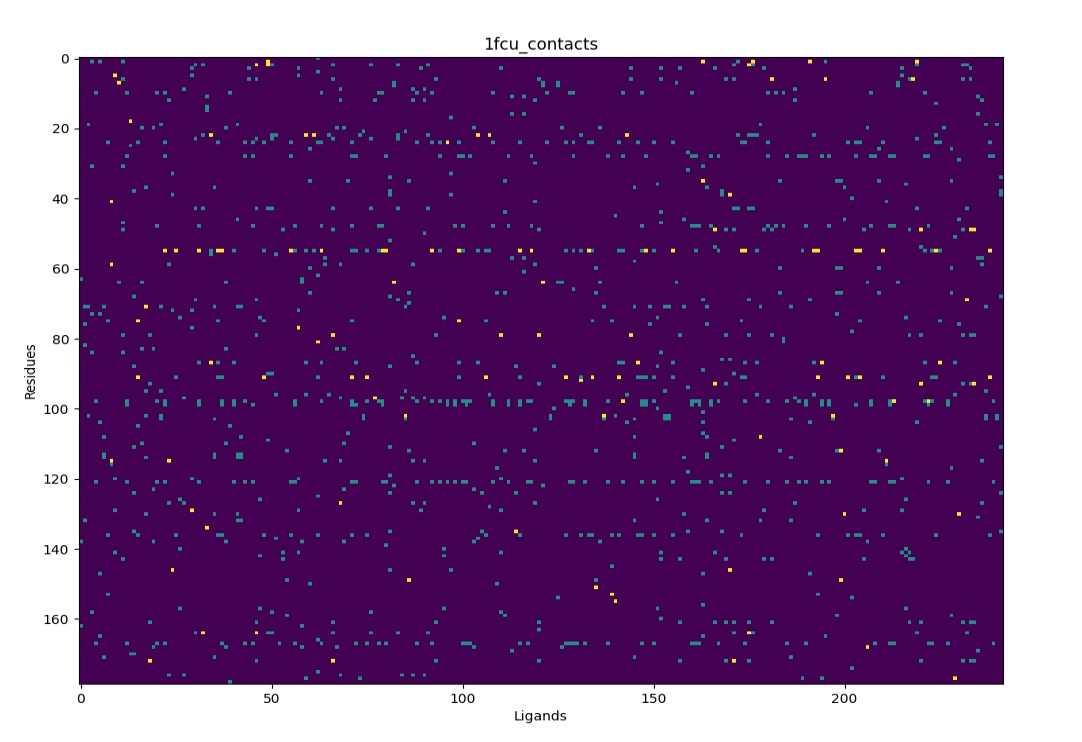
\includegraphics[width=\textwidth, height=6cm]{immagini/capitolo4/heatmap_gnina_1fcu.jpg}
        \caption[]%
        {{\small Heatmap delle interazioni per la proteina 1FCU prodotta a partire dalle pose predette dei ligandi da GNINA.}}    
        \label{fig:heatmap_gnina_1fcu}
    \end{subfigure}
    \hfill
    \begin{subfigure}[b]{\textwidth}  
        \centering 
        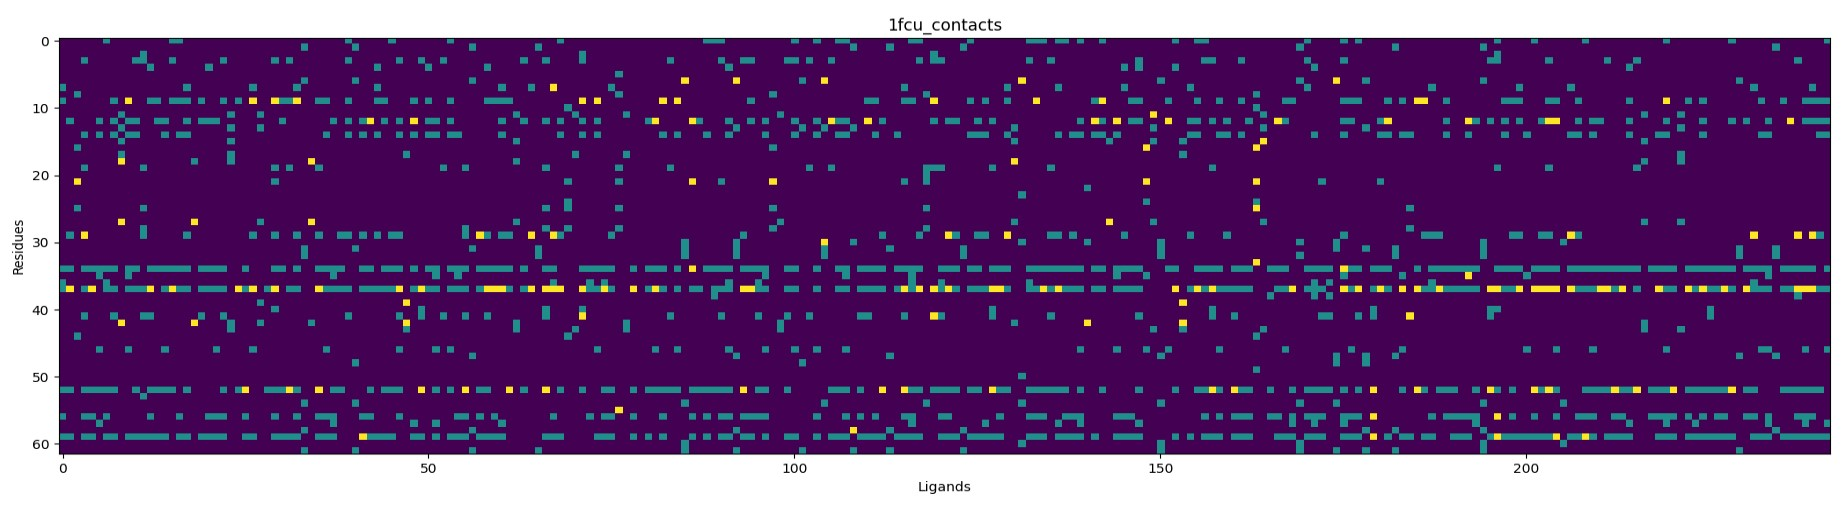
\includegraphics[width=0.9\textwidth, height=6cm]{immagini/capitolo4/heatmap_vina_1fcu.jpg}
        \caption[]%
        {{\small Heatmap delle interazioni per la proteina 1FCU prodotta a partire dalle pose predette dei ligandi da AutoDock Vina.}}    
        \label{fig:heatmap_vina_1fcu}
    \end{subfigure}
    \caption[Visualizzazione delle heatmaps per la proteina 1FCU.]
    {\small Visualizzazione delle interazioni per la proteina 1FCU attraverso heatmaps. In alto, è riportata l'heatmap risultante dalle pose predette da GNINA mentre in basso, quella risultante dalle pose predette da AutoDock Vina. Sull'asse delle ascisse sono riportati i ligandi, sulle ordinate i residui coinvolti per la proteina. In giallo sono riportati i legami a idrogeno, in azzurro/verde i close contacts, in viola nessun legame. } 
    \label{fig:1fcu}
\end{figure}
 
La Figura \ref{fig:1fcu} riporta le heatmaps prodotte dall'analisi delle interazioni molecolari relativamente alla proteina 1FCU per il dataset dei ligandi utilizzato (vedi Figura \ref{fig:heatmap_gnina_1fcu} per GNINA, vedi \ref{fig:heatmap_vina_1fcu} per AutoDock Vina).\newline
Si può osservare dalla tabella \ref{contacts_table} che GNINA ed AutoDock Vina operino sugli stessi dati, ma per quanto detto prima il riscontro è che le interazioni molecolari prodotte all'interno del complesso sono profondamente diverse. La visualizzazione delle heatmaps permette una conferma di quanto detto. 
Analizzando la Figura \ref{fig:heatmap_gnina_1fcu} che è relativa ai risultati di GNINA, è possibile notare come i residui coinvolti nell'intero processo superino le 100 unità, presentando inoltre una distribuzione più equa dei legami all'interno del complesso.\newline
AutoDock Vina produce risultati differenti per numero, in quanto i residui coinvolti sono circa 60 unità, e perchè le interazioni sono maggiormente concentrate in determinati residui: \textit{ARG244, SER225, TYR188, TYR190}.\newline 
Si può concludere che AutoDock Vina permette di distinguere più facilmente i residui che forniscono un apporto significativo da quelli il cui contributo è minimo, GNINA invece fa si che ogni residuo fornisca il proprio contributo in termini di interazioni.\newline
Questo tipo di situazione appare ancora più netta nel caso della proteina 5XZ3\_A, prendendo visione della Figura \ref{fig:5xz3_a}. 

\begin{figure}
    \centering
    \begin{subfigure}[b]{\textwidth}
        \centering
        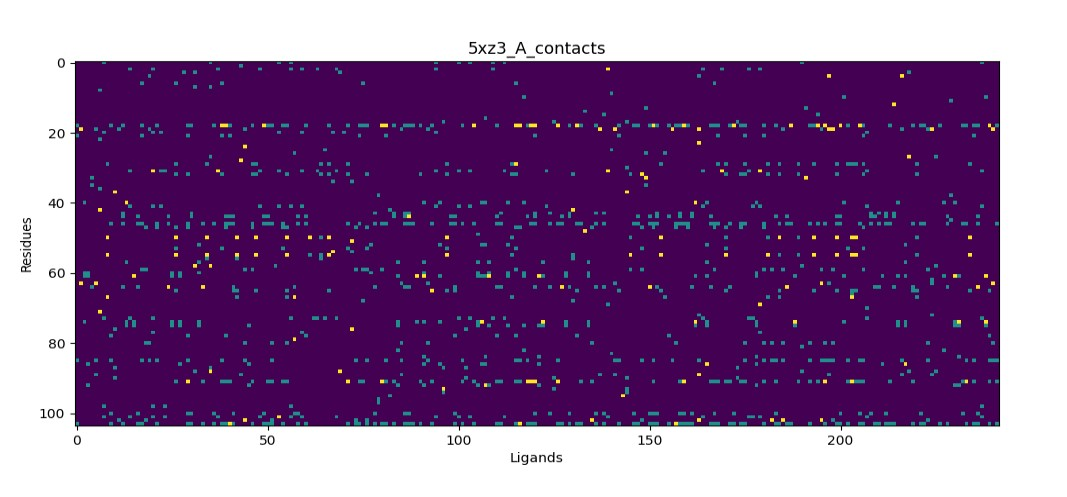
\includegraphics[width=\textwidth, height=6cm]{immagini/capitolo4/heatmap_gnina_5xz3_a.jpg}
        \caption[]%
        {{\small Heatmap delle interazioni per la proteina 5XZ3\_A prodotta a partire dalle pose predette dei ligandi da GNINA.}}    
        \label{fig:heatmap_gnina_5xz3_a}
    \end{subfigure}
    \hfill
    \begin{subfigure}[b]{\textwidth}  
        \centering 
        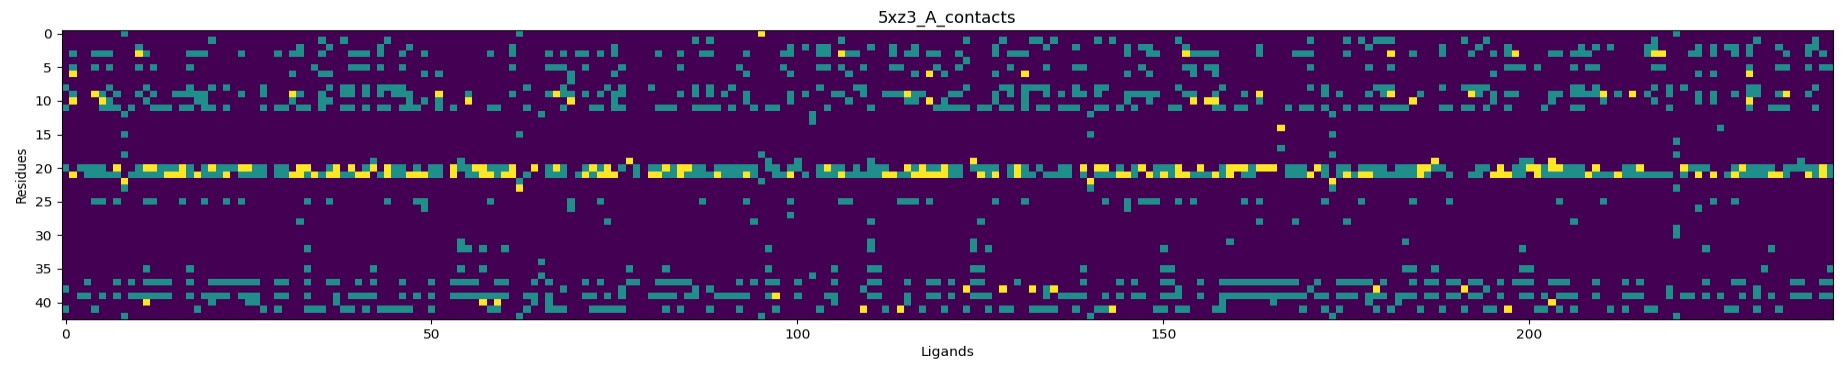
\includegraphics[width=0.9\textwidth, height=3cm]{immagini/capitolo4/heatmap_vina_5xz3_a.jpg}
        \caption[]%
        {{\small Heatmap delle interazioni per la proteina 5XZ3\_A prodotta a partire dalle pose predette dei ligandi da AutoDock Vina.}}    
        \label{fig:heatmap_vina_5xz3_a}
    \end{subfigure}
    \caption[Visualizzazione delle heatmaps per la proteina 5XZ3\_A.]
    {\small Visualizzazione delle interazioni per la proteina 5XZ3\_A attraverso heatmaps. In alto, è riportata l'heatmap risultante dalle pose predette da GNINA mentre in basso, quella risultante dalle pose predette da AutoDock Vina. Sull'asse delle ascisse sono riportati i ligandi, sulle ordinate i residui coinvolti per la proteina. In giallo sono riportati i legami a idrogeno, in azzurro/verde i close contacts, in viola nessun legame. } 
    \label{fig:5xz3_a}
\end{figure}

In questo caso però, la particolarità delle relative heatmaps sta nel fatto che nel caso della Figura \ref{fig:heatmap_vina_5xz3_a}, corrispondente ai risultati di AutoDock Vina, è possibile sintetizzare non solo la maggior parte delle interazioni in un sotto-insieme dei residui coinvolti, comunque minore in numero rispetto a quello evidenziato dalla Figura \ref{fig:heatmap_gnina_5xz3_a} relativa ai risultati di GNINA, ma anche la maggior parte dei legami a idrogeno prodotti in un sotto-insieme ancor più ridotto dei residui che compongono la proteina: \textit{HIS61, TYR72}.\newline
Le medesime considerazioni possono essere fatte ancor più intuitivamente visualizzando gli istogrammi relativi alle interazioni prodotte, i cui picchi individuano i residui maggiormente presenti nei legami. In basso sono riportati i residui che effettuano almeno un'interazione rilevanti; in blu è riportato il numero di close-contacts mentre in arancione il numero di legami a idrogeno per ciascun residuo proteico.

\begin{figure}
    \centering
    \begin{subfigure}[b]{\textwidth}
        \centering
        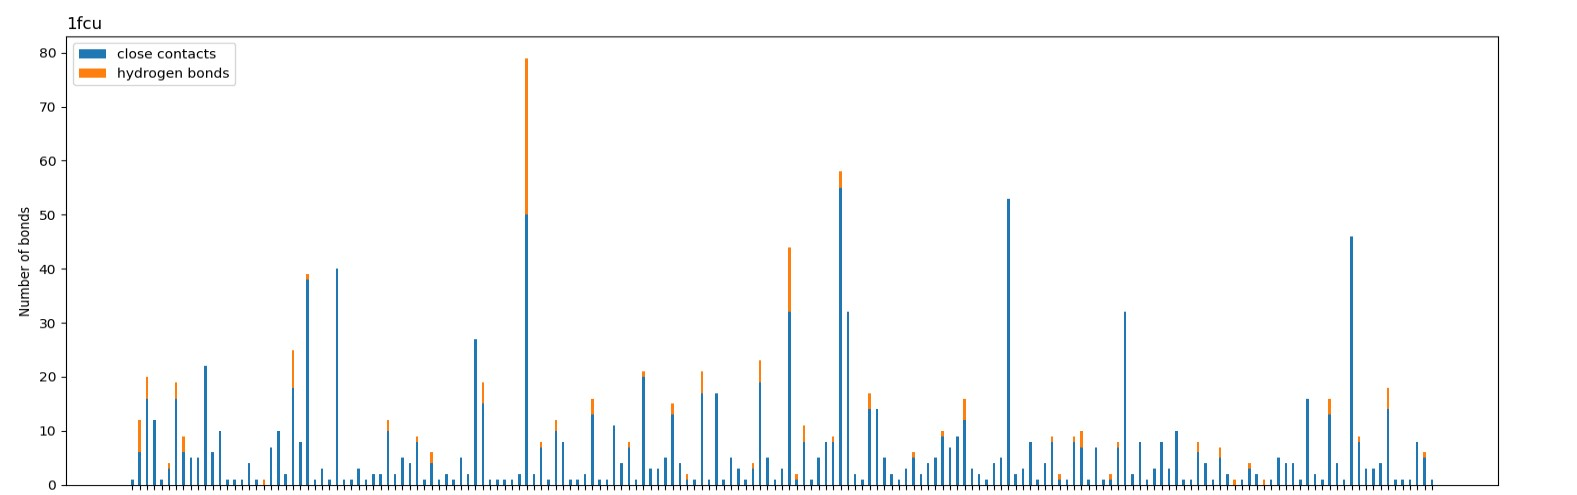
\includegraphics[width=\textwidth, height=6cm]{immagini/capitolo4/interactions_gnina_1fcu.jpg}
        \caption[]%
        {{\small Heatmap delle interazioni per la proteina 5XZ3\_A prodotta a partire dalle pose predette dei ligandi da GNINA.}}    
        \label{fig:interactions_gnina_1fcu}
    \end{subfigure}
    \hfill
    \begin{subfigure}[b]{\textwidth}  
        \centering 
        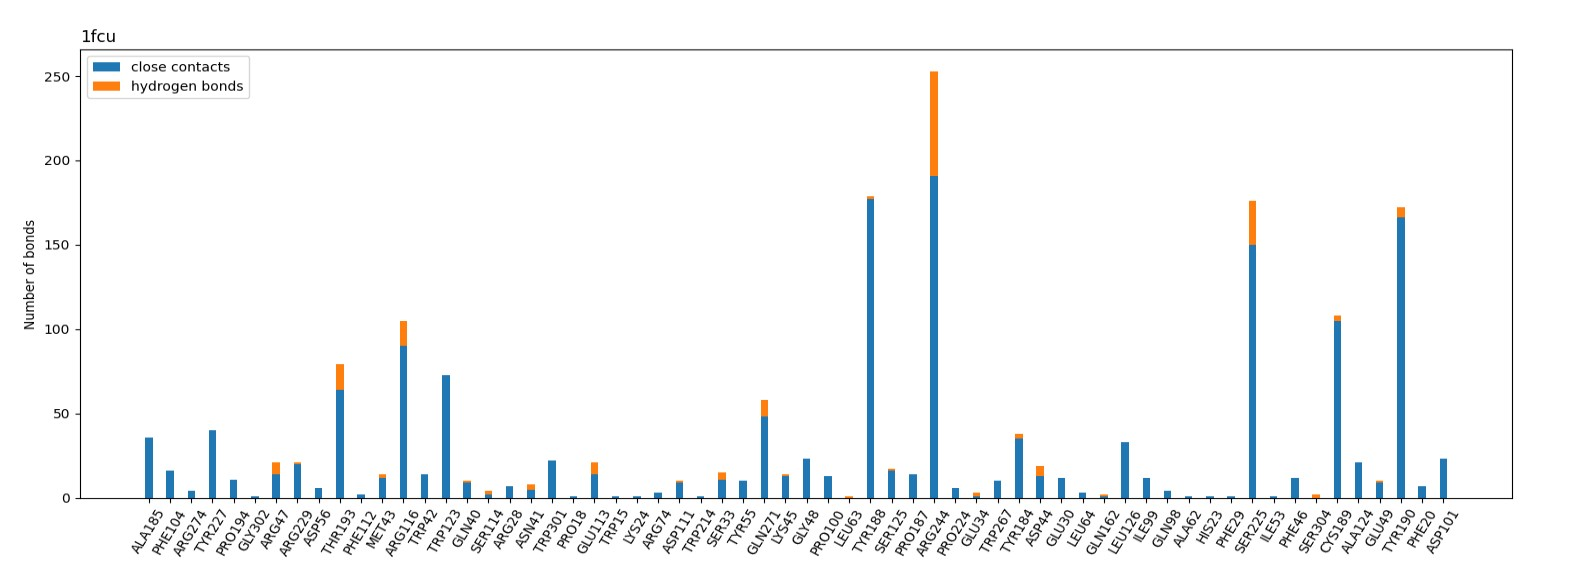
\includegraphics[width=0.9\textwidth, height=3cm]{immagini/capitolo4/interactions_vina_1fcu.jpg}
        \caption[]%
        {{\small Istogramma delle interazioni per la proteina 1FCU prodotta a partire dalle pose predette dei ligandi da AutoDock Vina.}}    
        \label{fig:interactions_vina_1fcu}
    \end{subfigure}
    \caption[Visualizzazione degli istogrammi per la proteina 1FCU.]
    {\small Visualizzazione delle interazioni per la proteina 1FCU attraverso istogrammi. In alto, è riportato l'istogramma risultante dalle pose predette da GNINA mentre in basso, quello risultante dalle pose predette da AutoDock Vina. Sull'asse delle ordinate è riportato il numero di contatti, sulle ascisse i residui coinvolti per ciascuna proteina. In arancione sono riportati i legami a idrogeno, in blu i close contacts. } 
    \label{fig:int_1fcu}
\end{figure}


\begin{figure}
    \centering
    \begin{subfigure}[b]{\textwidth}
        \centering
        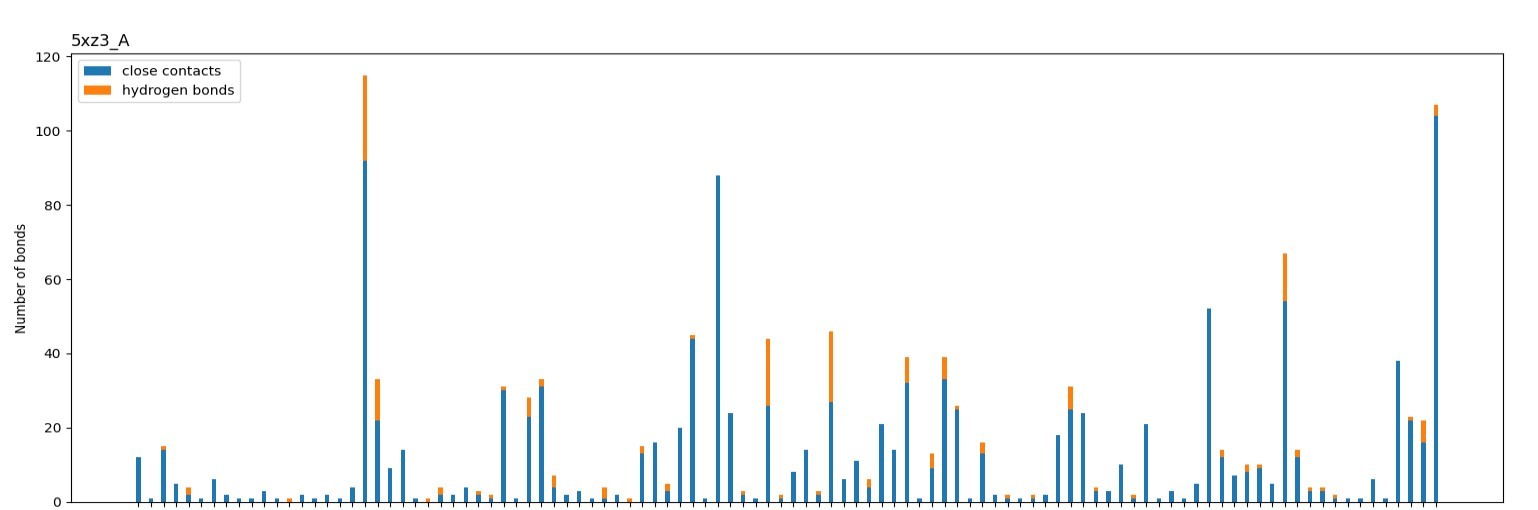
\includegraphics[width=\textwidth, height=6cm]{immagini/capitolo4/interactions_gnina_5xz3_a.jpg}
        \caption[]%
        {{\small Istogramma delle interazioni per la proteina 5XZ3\_A prodotta a partire dalle pose predette dei ligandi da GNINA.}}    
        \label{fig:interactions_gnina_5xz3_a}
    \end{subfigure}
    \hfill
    \begin{subfigure}[b]{\textwidth}  
        \centering 
        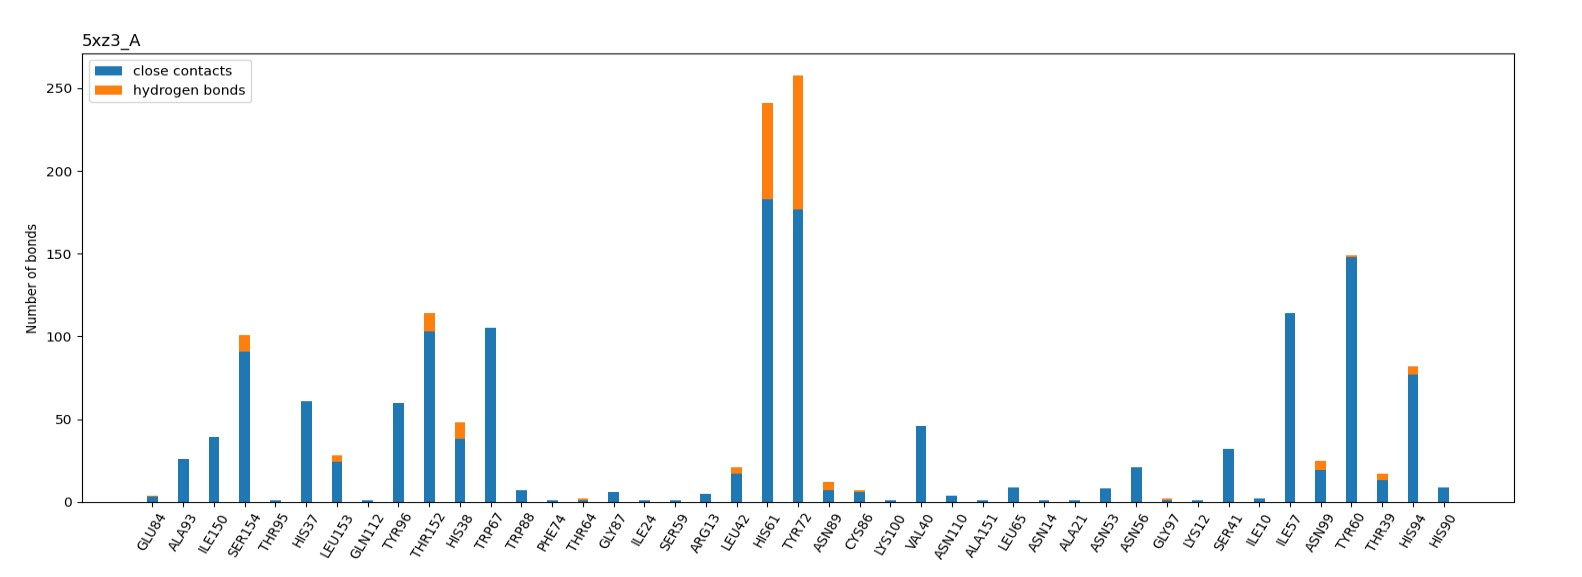
\includegraphics[width=0.9\textwidth, height=3cm]{immagini/capitolo4/interactions_vina_5xz3_a.jpg}
        \caption[]%
        {{\small Istogramma delle interazioni per la proteina 5XZ3\_A prodotta a partire dalle pose predette dei ligandi da AutoDock Vina.}}    
        \label{fig:interactions_vina_5xz3_a}
    \end{subfigure}
    \caption[Visualizzazione degli istogrammi per la proteina 5XZ3\_A.]
    {\small Visualizzazione delle interazioni per la proteina 5XZ3\_A attraverso istogrammi. In alto, è riportato l'istogramma risultante dalle pose predette da GNINA mentre in basso, quello risultante dalle pose predette da AutoDock Vina. Sull'asse delle ordinate è riportato il numero di contatti, sulle ascisse i residui coinvolti per ciascuna proteina. In arancione sono riportati i legami a idrogeno, in blu i close contacts.} 
    \label{fig:int_5xz3_a}
\end{figure}

In conclusione possiamo affermare che dal punto di vista delle interazioni molecolari, quelle prodotte da GNINA, sono quantitativamente inferiori ma qualitativamente migliori, rispetto a quelle prodotte da AutoDock Vina. Nonostante il numero di legami sia inferiore, è emerso che il numero di residui coinvolti in legami è notevolmente maggiore, producendo quindi heatmaps più ampie e sparse in cui le interazioni sono maggiormente distribuite, rispetto a quelle ridotte e fitte di AutoDock Vina, in cui è maggiormente possibile approssimare l'insieme dei residui coinvolti in interazioni ad un sotto-insieme ridotto di residui interessanti.

\section{Analisi dei tempi di esecuzione}
Per valutare le performance delle funzioni sviluppate, sono stati eseguiti 10 cicli incrementali per ciascuna funzionalità sviluppata, eccezion fatta per il docking la cui esecuzione con tutti i dati di input (289 ligandi, 11 recettori) presi in esame ha richiesto circa 3 giorni di esecuzione.\newline
Tutti i test sono stati eseguiti su \href{https://colab.research.google.com/}{Google Colaboratory} (Colab). Colab è una piattaforma gratuita che permette a chiunque di scrivere ed eseguire codice Python attraverso un browser. L’unico requisito è possedere un account Google (ad esempio Gmail). Colab è basato su un progetto Open Source chiamato \href{https://jupyter.org/}{Jupyter}. I documenti/programmi scritti su Colab sono chiamati Notebook e verranno salvati automaticamente sul Google Drive associato al proprio account.\newline
Le macchine virtuali messe a disposizione in Google Colab ospitano un ambiente configurato che consente di concentrarsi sin da subito sui progetti di Data Science:  sono presenti numerose librerie Python, tra cui moltissime di Data Science, si può usufruire di GPU e TPU per dare boost computazionali importanti ai lavori.\newline
Per facilitare la comprensione dei risultati ottenuti sono stati realizzati dei grafici, uno per ciascuna funzionalità testata.\newline
Ogni grafico riporta l'andamento dei tempi in funzione dell'incremento degli input relativi.\newline
Di seguito sono riportati i grafici relativi ai test effettuati per le funzioni:
\begin{itemize}
    \item Preparazione dei ligandi
    \item Preparazione dei recettori
    \item Esecuzione dell'analisi.
\end{itemize}

\begin{figure}[H]
    \centering
    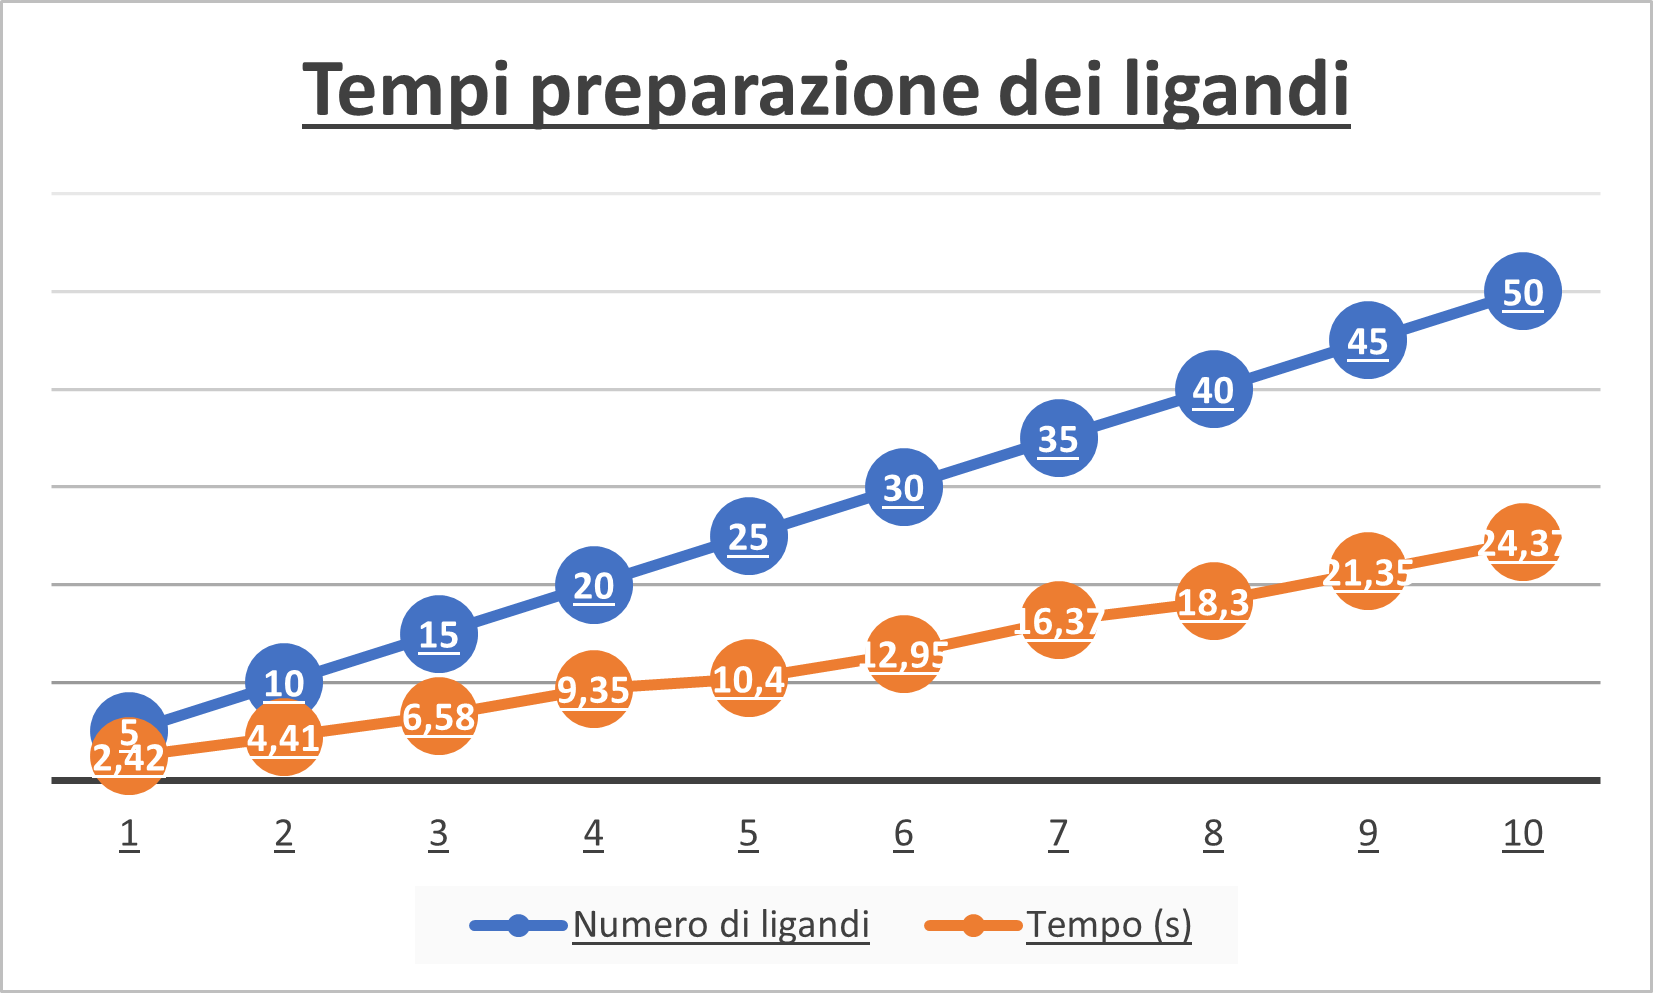
\includegraphics{immagini/capitolo4/tempiLigandi.png}
    \caption{Tempi di preparazione dei ligandi}
    \label{fig:tempi ligandi}
\end{figure}

\begin{figure}[H]
    \centering
    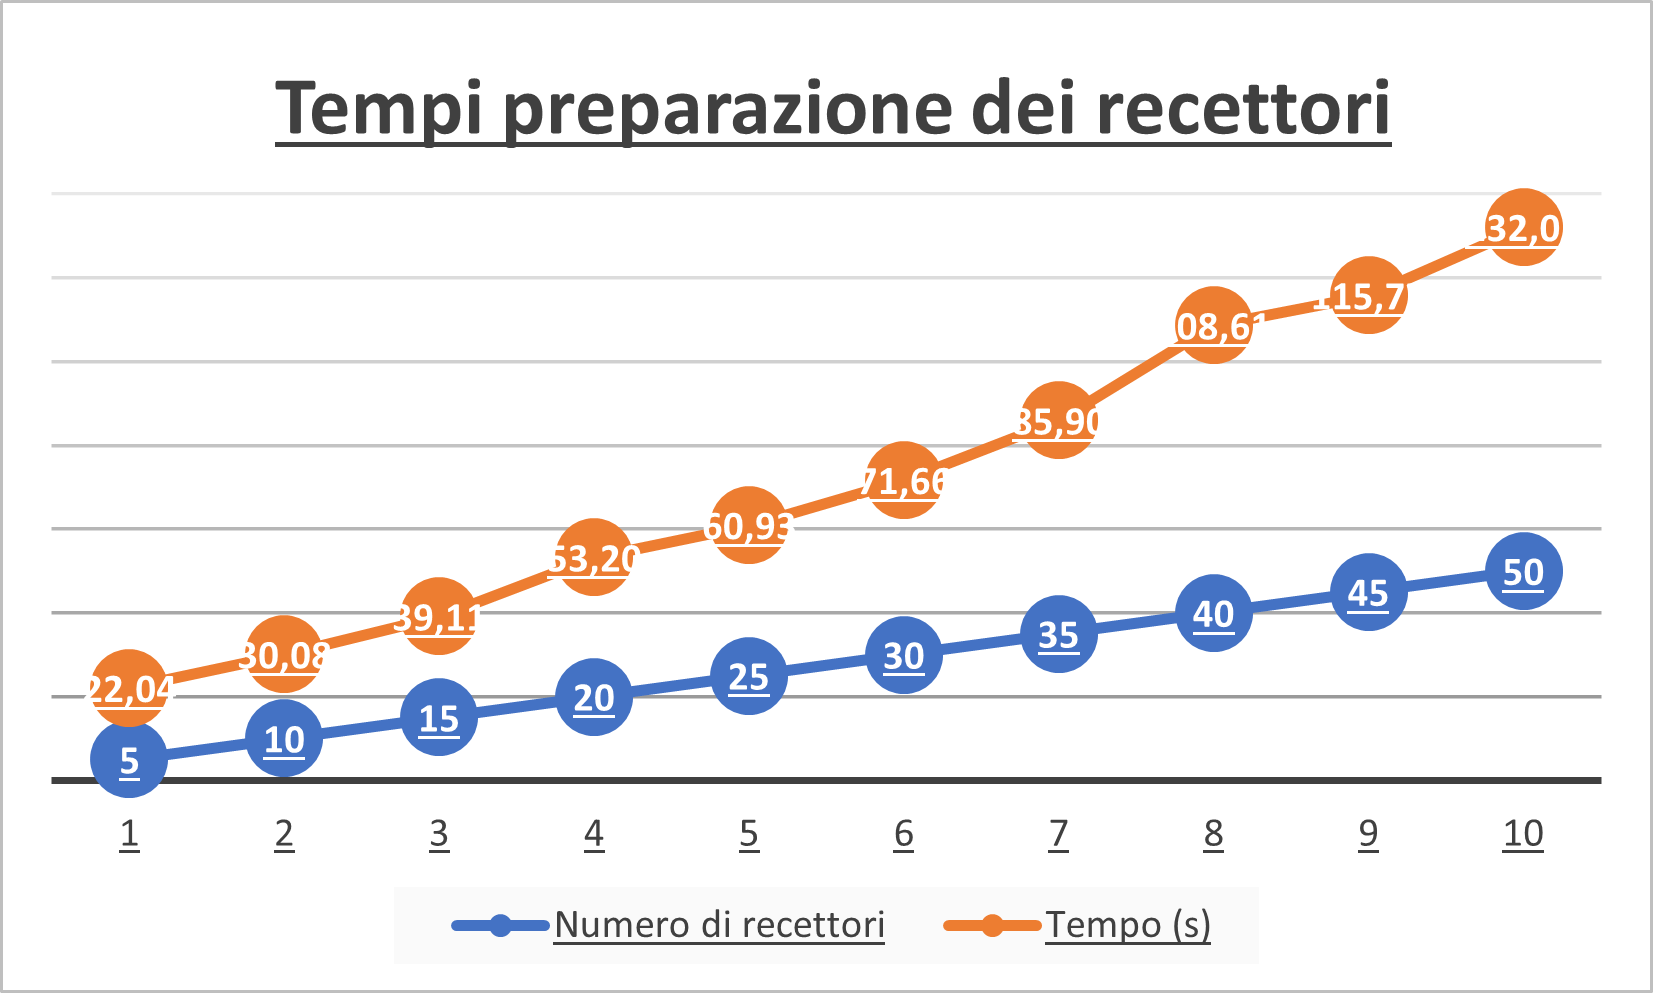
\includegraphics{immagini/capitolo4/tempiRecettori.png}
    \caption{Tempi di preparazione dei recettori}
    \label{fig:tempi recettori}
\end{figure}

\begin{figure}[H]
    \centering
    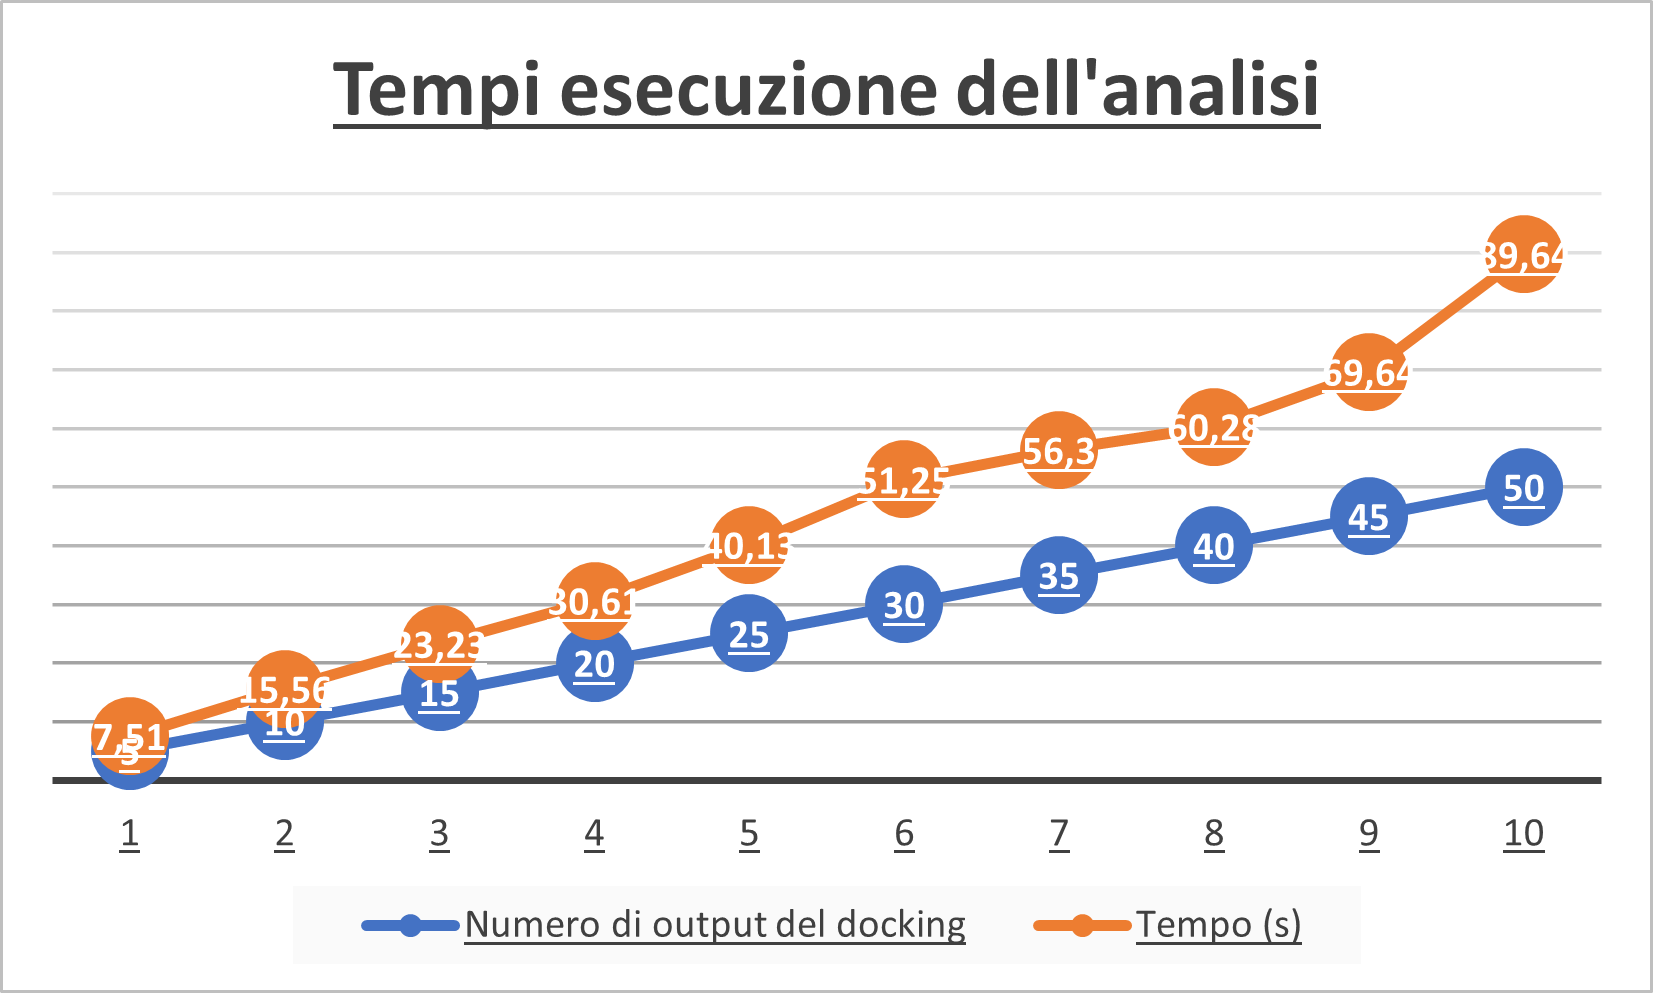
\includegraphics{immagini/capitolo4/tempiAnalisi.png}
    \caption{Tempi di esecuzione dell'analisi}
    \label{fig:tempi analisi}
\end{figure}

Osservando e comparando i dati dei grafici sopra, si può notare che:

\begin{itemize}
    \item le prestazioni delle funzioni, preparazione ligandi, preparazione recettori e analisi rispecchiano la stessa complessità di tempo
    \item le prestazioni del sistema in generale non degradano con il crescere dei dati in input
    \item l'andamento dei tempi si incrementa linearmente con l'aumentare dell'input.
\end{itemize}

\section{Comparazione con altri tools}
AUDO4RIAS è stato confrontato da un punto di vista di tempi di esecuzioni con un insiem di sofotware che eseguono le stesse funzionalità, quali:

\begin{itemize}
    \item \textbf{ADFR suite}, per la preparazione dei ligandi e dei recettori
    \item \textbf{GNINA}, per il Docking
    \item \textbf{AUTODOCKTOOLS}, per l'analisi dei risultati del dockig.
\end{itemize}

Nell'analisi comparativa effettuata, i tempi degli altri tools sono stati rilevati senza tener conto del tempo impiegato dall'utente per l'inserimento degli input per le integrazioni dei vari software, in quanto variabile da individuo ad individuo.\newline
I risultati ottenuti sono stati rappresentati nel seguente grafico:

\begin{figure}[H]
    \centering
    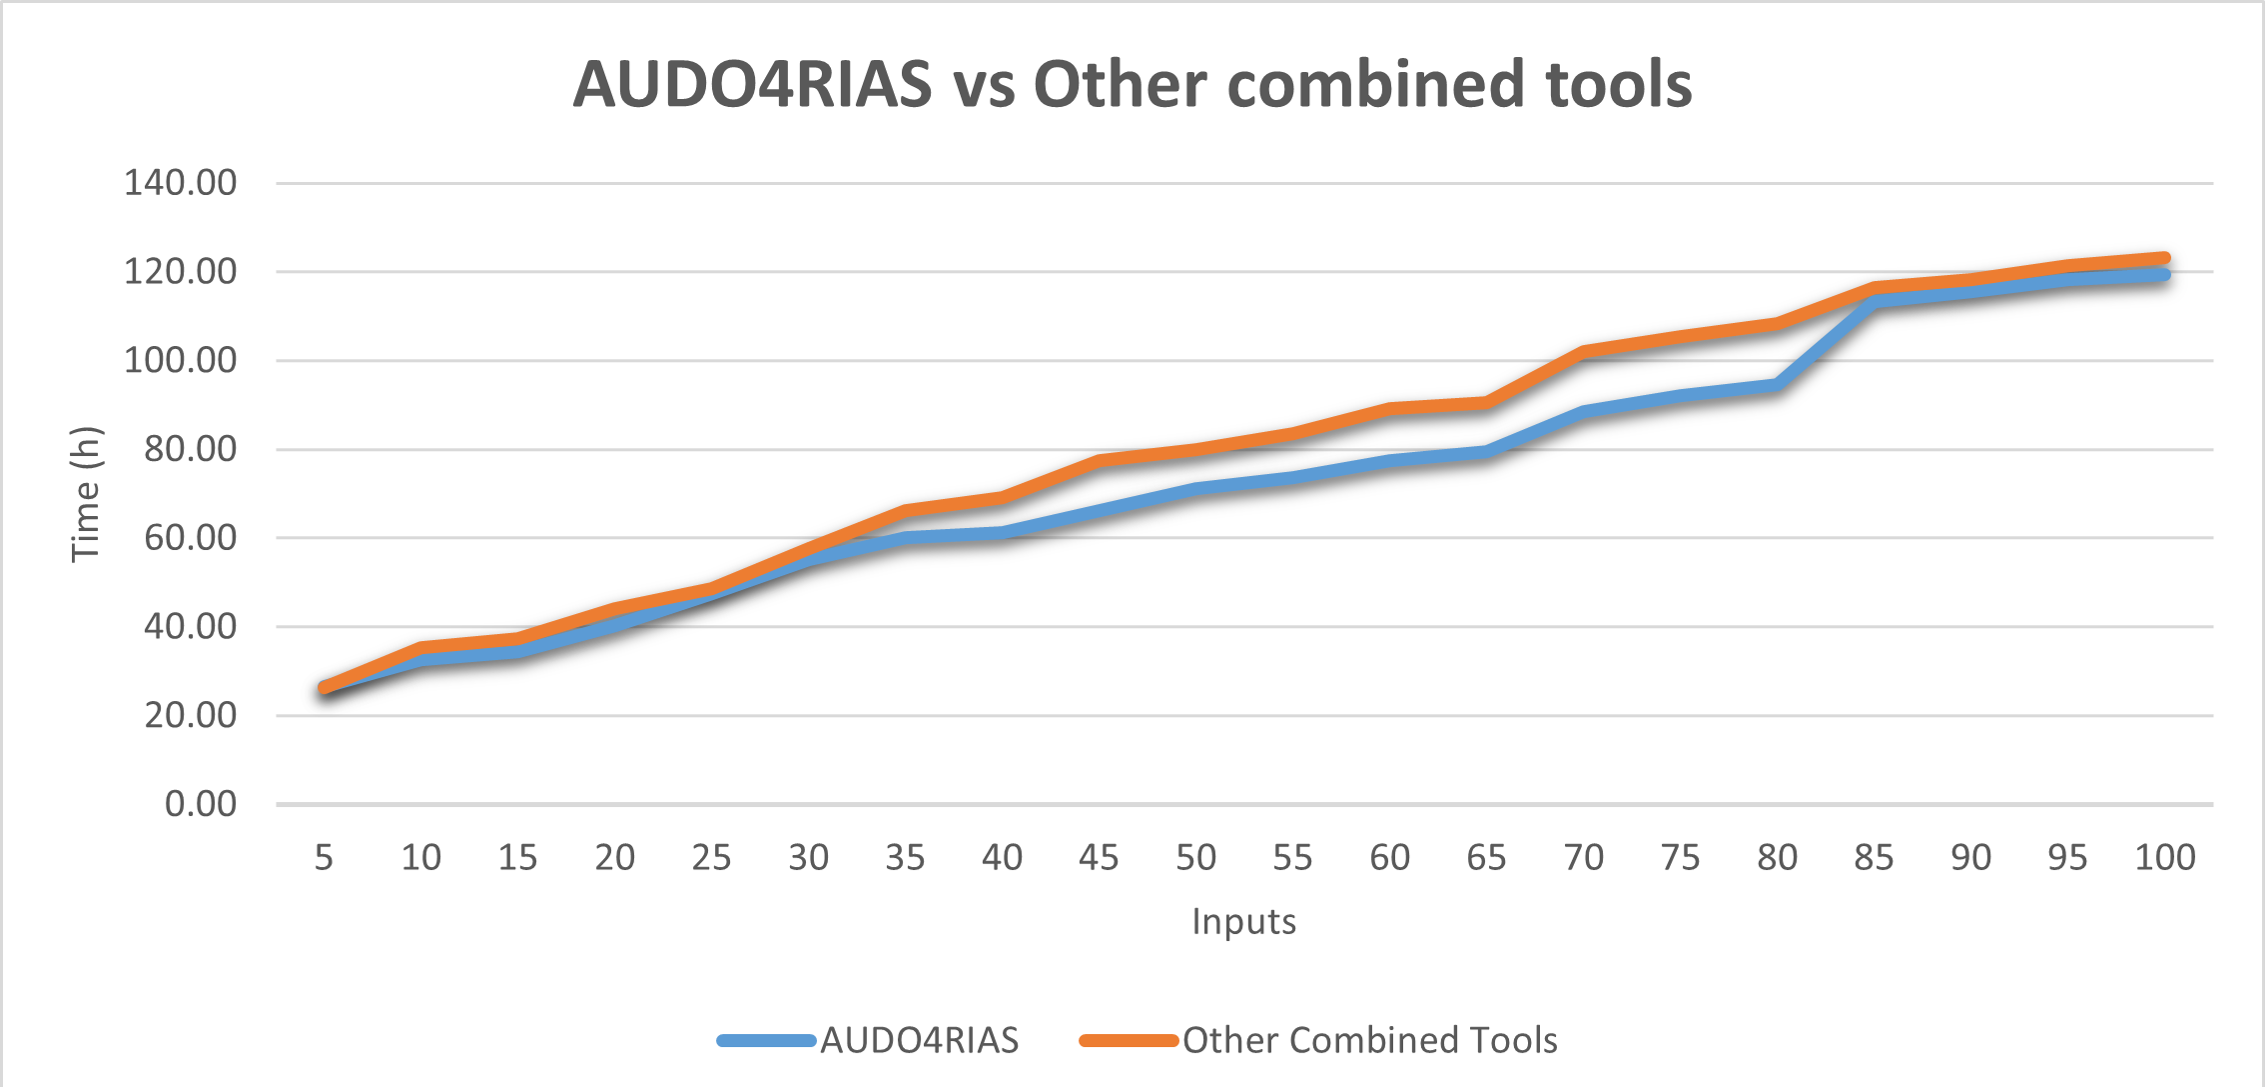
\includegraphics[scale=0.9]{immagini/capitolo4/comparazioneTempi.png}
    \caption{AUDO4RIAS vs other combined tools}
    \label{fig:comparazione tempi}
\end{figure}

Si può osservare che i tempi di AUDO4RIAS sono abbastanza in linea con quelli degli altri tool combinati, al netto del tempo impiegato dall'utente per le operazioni manuali intermedie necessarie necessarie durante l'utilizzo degli altri tools.\newline
Nell'analisi i tempi sono calcolate in ore e le elaborazioni per entrambi sono state effettuate su \href{https://colab.research.google.com/}{Google Colab}.